% 2023本郷祭 マイコン部 部誌 「マイコンHONGOMagazine」 TeXテンプレート

% =環境設定=

\documentclass[b5paper,10pt]{jsarticle}

% 数式
\usepackage{amsmath,amsfonts}
\usepackage{bm}

% 画像
\usepackage[dvipdfmx]{graphicx}

% 段組
\usepackage{multicol}
\setlength{\columnseprule}{0.5pt}

% 表(オリジナルパッケージ)
\usepackage{tabularx}

% 余白
\usepackage[paper=b5j,truedimen,margin=15truemm]{geometry}
\usepackage{ulem}
\usepackage{ascmac}

% ページ番号を削除
\pagestyle{empty}

% ソースコード環境
\usepackage{listings,jvlisting}
\usepackage{listings,jlisting}
\lstset{
  basicstyle={\scriptsize\ttfamily},
  identifierstyle={\scriptsize},
  commentstyle={\smallitshape},
  keywordstyle={\scriptsize\bfseries},
  ndkeywordstyle={\scriptsize},
  stringstyle={\scriptsize\ttfamily},
  frame={tb},
  breaklines=true,
  columns=[l]{fullflexible},
  numbers=left,
  xrightmargin=0zw,
  xleftmargin=0zw,
  numberstyle={\scriptsize},
  stepnumber=1,
  numbersep=1zw,
  lineskip=0.5ex
}
\renewcommand{\lstlistingname}{リスト}

% 書きたい内容に合わせてお好きなパッケージを導入していただいて構いませんが、外部パッケージは提出時に必ず合わせて提出してください。
% また、そのパッケージを使用している部分には必ずコメントをしてください。

% =環境設定ここまで=

\begin{document}

% =タイトル=
\title{書店で見かけたScratchの入門書が簡単すぎるので\\誰からも頼まれていませんが\\勝手にScratchについて解説します。}
\author{TurboWarp狂の副部長}
\date{\today}
\maketitle
% 初めのページのページ番号を削除(\maketitleの影響を回避)
\thispagestyle{empty}

% ここではページごとに段組しています。大きく画像を表示したいときなどは以下を \begin{multicols}{3} 、\end{multicols}のように変更すると文章が終わった直後から空白になります
\begin{multicols*}{3}
  
% 以下本文
皆さんこんにちは。Scratchを(おそらく)極めた、やる気が出ない副部長です。タイトルが一部のああいうラノベのように長いですね。この記事では今後も長ったらしい文、また文法がおかしい文、読みにくい文がずっと登場しますので苦手な方は次の記事へ進んでくれてかまいません。

さて、本題に入ります。いつのことだか忘れましたが、私がUnityとCsharpについて学び始めたころ(たったのおよそ1、2ヶ月前ですね)、それに関する参考書がないかな~と近くの書店の「プログラミング」というコーナーに寄りました。いい感じの解説書は無事手に入りましたが、とある参考書が私の目に留まったんですよね。そう、今回の本題のきっかけ(悪口・愚痴の対象でもある)となったScratchの参考書です。その場でパラパラとめくってみました。簡単。簡単すぎる。読み応え0。つまらないので別の参考書も手に取ってみました。説明は省略します。これでは実力のあるScratcher(Scratchをする人)は生まれません。\sout{だから今のScratchは\\民度が低いわけですね。}\\だからScratchが得意という人が少ないんですね。

というわけで前置きが馬鹿みたいに長くなりましたが、今回はScratchの概要、基本的な機能、参考書で語られていない部分、闇の部分を\sout{さらけ出して}紹介して行きたいと思います。皆さんの待ちに待った目次をどうぞ。

\begin{itembox}{目次}{1. }scratchの基礎知識\\{ a. }概要\\{ b. }Scratchの機能・ブロック\\{ c. }外部MODのTurbowarp\\{2. }制作\\{ a. }使用例\\{ b. }作品例\\{ c. }Turbowarpの素晴らしいところ
\end{itembox}

\section{Scratchの基礎知識}
\subsection{概要}
まずScratchとはいったい何なのか。まあこのような説明が必要な方は基礎を一から学ばれた方がよろしいと思うので、ぜひ書店に足を運ぶなり、ネットで記事を読むなりしたほうが分かりやすく学べると思いますが、この章ではそんな時間や余裕のない方のために、簡単に説明をしていこうと思います。

Scratchは一種のプログラミング言語であり、その非常にわかりやすいUI、手軽な操作により様々な教育現場で使われています。あいにく本郷では講座はありません。Scratchの仕組みとしては、「スプライト」と呼ばれる2Dのオブジェクトを編集しステージ上で動かすというのがメインです。エディター画面(図1)にて、左側のパレットからブロックをドラッグ&ドロップしてスクリプトを組み立てていったり、「コスチューム」とよばれるスプライトのスキンを編集したりするといった感じです。
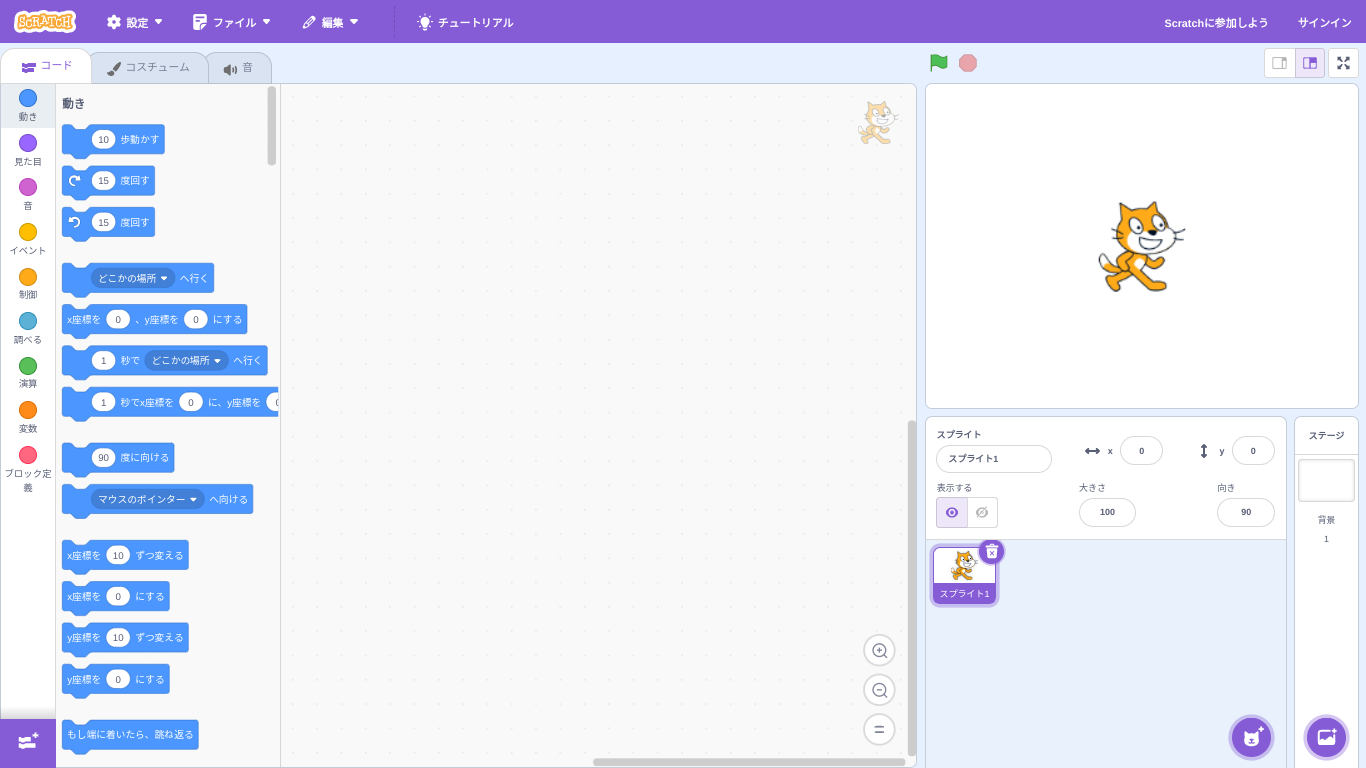
\includegraphics[width=4cm]{editor.png}図1\\
組み立てたスクリプトは、クリックするか、「旗が押されたとき」というイベントカテゴリ(後述)のブロックを先頭にくっつけてステージの上の緑色の旗を押すと実行されます。
少し細かい話をしますと、ScratchはJavaScriptで記述されており、30fpsで動きます。また、拡張機能を使うとLEGOと連動したり、カメラで動きを検知したりすることもできます。

まあ、こんな感じでScratchはキーボードがなくてもマウスだけでプログラミングができるという破格の性能(無料だけど)をしています。
\subsection{TurboWarpとは}
ここからは布教活動となりますので、興味のない方は飛ばしてもらって結構です。

それではまず皆さん唱えましょう。
% ソースコードを見ているあなたも唱えましょう。
Repeat after me.
TurboWarp(ターボワープ)は神です。

TurboWarpはGarboMuffin氏によって製作されたScrtachのModです。UI、操作方法、仕組みなどはほぼ同じですが、TurboWarpはプロジェクトの軽量化に加え、フリーズ・クラッシュ防止のWarpタイマー、FPSの変更、Scratchにおけるさまざまな制限を解除できる設定など、Scratchと比べて機能が非常に充実しています。さらに、アドオンの設定では、一時停止ボタン、変数マネージャー、ブロックのドロップダウン検索などと地味ですがとてもうれしいっ機能も盛りだくさんです。
また、最近知ったのがTurboWarpの独自の拡張機能(紛らわしいですがアドオンとは別物です)ですが、異常なほど多く、Scratchに既にあるアナログな拡張機能に加え、
Gamepad(ゲームコントローラを連携できる)、
Files(ファイルのインポート・エクスポートができるブロックを追加)、
Runtime Option(通常は自分でいじる必要のある環境設定をスクリプトから調整することが可能)、
Sensing+やClone+やLook+(「調べる」や「見た目」というカテゴリとクローン関連のブロックを追加)、
Clipping&Blending(画像の切り抜きや描写に関する調整が可能)、
Local Storage(ほぼCookie)などと言い足りませんが様々なものがあります。
ちなみに執筆時点でおよそ80個で、まだまだ増えています。
そして、それらのほとんどはまさに「痒い所に手が届く」な便利な機能です。まだScratchをお使いの方はぜひTurboWarpへの乗り換えをご検討ください。TurboWarpはScratchと同じ形式でプロジェクトをインポート・エクスポートできるので、データの移動はとても簡単です。

\section{Scratchのブロック}

さて、お次はScratchの機能とそれに関連するブロックについてみていきましょう。先ほどお伝えした通り、Scratchはブロックをドラッグ&ドロップしてスクリプトを組み立てていくのですが、書店の参考書にはそれぞれのブロックに対する詳細な説明がありませんでした。これは減点ですね。ということでここからScratchのすべてのブロックとそのカテゴリに対して説明していこうと思うのですが、Scratchはブロックが多く\sout{面倒くさい}スペースがあまりないので、以降、ブロック、使用頻度、説明の順番で簡単に説明していきます。それでは、\\
 _______\\
/│  Hmcc │\\
││ (* '▽') │\\
││  舞昆布 │\\
 ̄ ̄ ̄ ̄ ̄ ̄ ̄ ̄\\
ゆっくりしていってね!!\\
↑モニターマン in LATEX

\pagebreak
\subsection{動き}
動きカテゴリは主にそのスプライトの座標、角度について制御するブロックの集まりです。基本的で直感的に理解しやすいブロックだらけです。

\begin{itembox}{1}
(n)歩動かす
\end{itembox}
使用頻度×\\
そのスプライトが現在向いている方向に向かって座標をxだけずらす。たとえば、スプライトの向き=30°、n=2のとき、このブロックを実行するとx座標が√3、y座標が1変わる。ぶっちゃけ使わない。
\begin{itembox}{2}
(n)度回す
\end{itembox}
使用頻度○\\
そのスプライトの現在の向きをnだけ変える。デフォルトで90°。また、時計回りとその逆で2つブロックがありるが、負の値もちゃんと読み取ってくれて動作するのでただただ無駄なだけ。なんで2個もあるんだ?
\begin{itembox}{3}
(どこかの場所▽)へ行く
\end{itembox}
使用頻度×\\
このブロックを実行することで、ランダムな場所に行ったりほかのスプライトやマウスに座標を合わせることができる。代用できるので使わない。
\begin{itembox}{4}
x座標を(n1)、y座標を(n2)にする
\end{itembox}
使用頻度△\\
xとy座標を変更できるブロック。個別に変更できるほかのブロックがあるので正直いらない。あと個人的にキモい。
\begin{itembox}{5}
(n)秒で(どこかの場所▽)へ行く
\end{itembox}
使用頻度×\\
「どこかの場所へ行く」の秒数がついたバージョン。座標で事足りるっつってんだろうが。
\begin{itembox}{6}
(n)秒でx座標を(n1)に、y座標を(n2)に変える
\end{itembox}
使用頻度△\\
少しまともなやつ。FPSに影響されないので、ラグいプロジェクトやTurboWarpでFPSを変更したプロジェクトで使えるかも。基本代替可。あとキモい
\begin{itembox}{7}
(n)度に向ける
\end{itembox}
使用頻度○\\
スプライトの向きを指定する。使うときはめちゃくちゃ重宝する。自分は最近使っていない。
\begin{itembox}{8}
(マウスのポインター▽)へ向ける
\end{itembox}
使用頻度×\\
座標&三角関数で物足りる。はい。
\begin{itembox}{9}
x座標を(n)ずつ変える\\y座標を(n)ずつ変える
\end{itembox}
使用頻度◎\\
プライトのxy座標の移動は主にこれを使う。これらのブロックのせいでほかのいくつものブロックが死んだ。とても優秀
\begin{itembox}{10}
x座標を(n)にする\\y座標を(n)にする
\end{itembox}
使用頻度◎\\
スプライトの座標の指定。位置の初期化、指定場所への移動などはこれを使う。めちゃくちゃ優秀。
\begin{itembox}{11}
もし端についたら、跳ね返る
\end{itembox}
使用頻度×\\
謎ブロック。実行された時点でステージの端にぶつかったとき、ぶつかった場所に応じてx軸またはy軸で向きを反転する。ほんとに謎。
\begin{itembox}{12}
回転方法を[左右のみ▽]にする
\end{itembox}
使用頻度△\\
左右のみ、回転しない、自由に回転の3つから選べる。左右のみの場合、0°~179°はそのまま、180°(-180°)~359°(-1°)はコスチュームの左右が反転した状態解いて反映される。それ以外の2つは字面通り。
\begin{itembox}{13}
(x座標)\\(y座標)
\end{itembox}
使用頻度◎\\
このスプライトの現在の座標を出力する引数。他スプライトの座標を取得するときは調べるカテゴリのブロックが使えるが、正直これで代用できる
\begin{itembox}{14}
(向き)
\end{itembox}
使用頻度△\\
このスプライトの向きを出力。正直変数を作ったほうが管理しやすい。

\subsection{見た目}
見た目カテゴリは、コスチュームの描写、レイヤー、大きさに関連したブロックと、一部の「なぜここに分類したのかブロック」を含みます。横・縦のみの伸縮ができるブロックをずっと求めていましたが、そんな拡張機能が最近TurboWarpに追加されました。控えめにいって神ですね。

\begin{itembox}{1}
(こんにちは!)と(n)秒言う
\end{itembox}
使用頻度×\\
こんなブロック、このカテゴリに入れちゃっていいんですか?
\begin{itembox}{2}
(こんにちは!)と言う
\end{itembox}
使用頻度×\\
本当にこのカテゴリに入れちゃっていいんですか??
\begin{itembox}{3}
(うーん...)と(n)秒考える
\end{itembox}
使用頻度×\\
運営さん、このブロックはこのカテゴリに属していると思っているんですか???
\begin{itembox}{4}
(うーん...)と(n)秒考える
\end{itembox}
使用頻度×\\
まじめな話をすると、一応リアルタイムで何かの値をモニターすることはできます。代替可なのでほぼ意味なし。枠のデザイン変更出来たらまだ使い道はあったんですけどね。ちなみにTurboWarpの拡張機能に、これのほぼ上位互換であるAnimated Textなるものがございまして...
\begin{itembox}{5}
コスチュームを(costume▽)にする
\end{itembox}
使用頻度◎\\
スプライトのコスチュームを変更するときに欠かせない。
\begin{itembox}{6}
次のコスチュームにする
\end{itembox}
使用頻度○\\
「前のコスチュームにする」ブロックもください。そうしたらもっと使ってやりますよ。
\begin{itembox}{7}
背景を(背景1▽)にする、次の背景にする
\end{itembox}
使用頻度×\\
背景はステージのスキンを指します。そもそもステージを背景目的で使うことなんてめったにないのでお役御免です。
\begin{itembox}{8}
大きさを(n)ずつ変える

大きさを(n)%にする
\end{itembox}
使用頻度◎\\
スプライトの大きさを制御できる唯一のブロック。10000%とかにすると当たり判定がおかしくなることがあるので要注意。
\begin{itembox}{9}
[色▽]の効果を(n)ずつ変える

[色▽]の効果を(n)にする
\end{itembox}
使用頻度○\\
ドロップダウンメニューから選んだ画像効果をかける。色、明るさ、透明度などよく見る効果や渦巻、魚眼レンズなど使い道がよくわからない効果がたくさんある。
\begin{itembox}{10}
画像効果をなくす
\end{itembox}
使用頻度○\\
一個上のブロックでかけた画像効果をすべて解除。効果をかけまくって何が何だか分からなくなったときに使う。
\begin{itembox}{11}
表示する\\隠す
\end{itembox}
使用頻度◎\\
スプライトを表示・非表示にしてくれる。見えてほしくないスプライトはこれで隠しましょう。
\begin{itembox}{12}
[最前面▽]へ移動する

(n)層[手前に出す▽]
\end{itembox}
使用頻度○\\
Scratchにはレイヤーの概念が存在しており、レイヤーidが大きい方が前面に表示されます。また、1レイヤーにつき1スプライトまでしか配置できません。レイヤーの調節に関しては、TurboWarpの拡張機能「Looks+」を使うことをお勧めします。
\begin{itembox}{13}
(コスチュームの[番号▽])
\end{itembox}
使用頻度○\\
ドロップダウンメニューから読み取るものを番号か名前か選択できます。このブロックのおかげでコスチューム名をデータを入れる場所として使うことができます。これは余談ですが、ScratchはコードではaとAを区別できないのに、コスチューム名では区別できます。
\begin{itembox}{14}
(背景の[番号▽])
\end{itembox}
使用頻度×\\
いうまでもないですね。もはやスペースの無駄
\begin{itembox}{15}
(大きさ)
\end{itembox}
使用頻度△\\
(向き)同様変数を作った方が管理しやすいのであまり使わない。

\subsection{音}
音カテゴリはそのまま音に関するブロックの集まりです。特にこれ以上言うことはないですね。
\begin{itembox}{1}
終わるまで(sound▽)の音を鳴らす
\end{itembox}
使用頻度○\\
音が鳴り終わるまで処理が終わらないので、特に音楽(bgm)を流すときは「ずっと」ブロックと相性がいいので重宝する。
\begin{itembox}{2}
(sound▽)の音を鳴らす
\end{itembox}
使用頻度○\\
音を垂れ流したまま次のブロックが処理される。おもに短い効果音などそのまま垂れ流されても困らない場合、または次のブロックが重要で迅速に処理されるべき場合に使う。
\begin{itembox}{3}
すべての音を止める
\end{itembox}
使用頻度○\\
ほかのスプライトが鳴らしている音もすべて止めるので要注意。
\begin{itembox}{4}
[ピッチ▽]の効果を(n)ずつ変える

[ピッチ▽]の効果を(n)にする
\end{itembox}
使用頻度○\\
ドロップダウンメニューからピッチ、「左右にパン」を選択可能。0でデフォルト。ちなみにピッチを120に設定することでおよそ2倍速、70でおよそ1.5倍速。また-infinityに設定することで(TurboWarpの高度な設定でその他の制限を解除する必要があり)音を一時停止することもできます。Scratchは無理なのでぜひTurboWarpを。
\begin{itembox}{5}
音の効果をなくす
\end{itembox}
使用頻度△\\
「画像効果をなくす」の音版。ピッチのリセットは自分で0に設定したほうがなんとなくすっきりするのであまり使わない。
\begin{itembox}{6}
音量を(n)ずつ変える

音量を(n)%にする
\end{itembox}
使用頻度△\\
音量はスプライトごとに違うので注意。
\begin{itembox}{7}
(音量)
\end{itembox}
使用頻度△\\
(向き)と(大きさ)と同じなので割愛。

\subsection{イベント}
さあやってきました、Scratchにて最も重要といえるかもしれないイベンカテゴリです。イベントカテゴリでは、例えば「緑の旗が押された」とか、「メッセージを受け取った」などのイベントをトリガーに、その後ろにくっついているブロックを活性化させます。このカテゴリがなきゃScratchは動きません。なぜなら先頭にイベントカテゴリンのブロックがついていないスクリプトは自動的に動作しないからですね。
\begin{itembox}{1}
旗が押されたとき
\end{itembox}
使用頻度 ほぼ必須◎◎\\
これがなきゃScratchは始まらない!ぐらいに重要で初心者のころからずっと使っているであろうブロック。今更解説する必要などないでしょう。
\begin{itembox}{2}
[スペース▽]キーが押されたとき
\end{itembox}
使用頻度○\\
おそらくあなたも初心者のころに使ったであろうブロック。ほかの条件と組み合わせる場合<(スペース▽)キーが押された>で事足りますが、イベントとして使うときはやはりこのブロックがしっくりきます。ちなみにTurboWarpのアドオンで「キー入力オプションの追加」をONにすることで、ctrlやshift、Enterや記号キーを感知できるようになります。
\begin{itembox}{3}
このスプライトが押されたとき
\end{itembox}
使用頻度△\\
「押されたとき」という条件はめちゃくちゃ使うんですけどこれじゃあほかの条件(例えば変数が特定の値の時のみ)とうまく組み合わせることができないんですよね。なので基本的には<<マウスが押された>かつ<(マウスのポインター▽)に触れた>>で代用することになります。
\begin{itembox}{4}
背景が[背景1▽]になったとき
\end{itembox}
使用頻度×\\
背景は使わない。
\begin{itembox}{5}
[音量]>(n)のとき
\end{itembox}
使用頻度○\\
ドロップダウンメニューから音量かタイマーか選べる。一部のイベントブロック(例えばこれ)は、コードペイン(コードを組む場所)に出しただけで常時プログラムが走っている状態になります。赤丸を押しても止まりません。しかし、条件を満たさない限りは実際にはただの見た目の問題なので気にしないでください。ちなみに小技として、タイマー>0を利用すると、実質的に「赤丸が押されたとき」というブロックを再現することができます。知らない人はぜひチャレンジしてみてください。
\begin{itembox}{6}
[メッセージ1▽]を受け取ったとき
\end{itembox}
使用頻度◎\\
メッセージは主にスプライト間でのタイミングのやり取りに使われます。普通に便利
\begin{itembox}{7}
[メッセージ1▽]を送る

[メッセージ1▽]を送って待つ
\end{itembox}
使用頻度◎\\
便利。「送って待つ」のほうは、メッセージを受け取ったスプライトが処理を完了するまで次のブロックに進めないので、受け取るスプライトに先に必要な処理をさせる場合に使える。有能。

\subsection{制御}
やってまいりました。イベントカテゴリと並ぶほど重要なやつ、それが制御カテゴリです。これを自由自在に使いこなせれるのが中級者(と勝手に思っています)ので、頑張ってマスターしましょう。

\begin{itembox}{1}
(n)秒待つ
\end{itembox}
使用頻度◎\\
初心者の頃は特にお世話になったブロックの一つ。タイミングの調整にめちゃくちゃ使えます。豆知識ですが、正確な秒数はn=1で約1.020秒(パフォーマンスにもよりますが私の場合は1.017~1.023秒でした)、n=0で約0.033秒(=30fpsのときの1フレーム)ですちなみに何も入力しなくてもn=0として認識されます。
\begin{itembox}{2}
(n)回繰り返す{}
\end{itembox}
使用頻度◎\\
もはや解説などいりませんね。こんな使いやすいブロック。ちなみに小技ですが、「このクローンを削除する」を「1回繰り返す」で挟むとスクリプトの途中でクローンを全消ししてメインのスプライトだけ処理を継続することもできちゃいます。
\begin{itembox}{3}
ずっと{}
\end{itembox}
使用頻度◎\\
ずっと繰り返したい処理に対して使う。条件付きの場合は中にほかのブロックを挟むといい
\begin{itembox}{4}
もし<>なら{}
\end{itembox}
使用頻度◎\\
条件分岐第一弾。if-。特定の条件を満たしたときのみこのブロックで囲んだブロックを処理する。
\begin{itembox}{5}
もし<>なら{}でなければ{}
\end{itembox}
使用頻度◎
条件分岐第二弾。if-else-。重ね掛け(elseの部分にまたif-else-を入れる繰り返し)すると見た目が悪くなるが機能性は素晴らしい。
\begin{itembox}{6}
<>まで待つ
\end{itembox}
使用頻度◎\\
何かの条件がそろうまで次の処理に移らない。タイミング合わせや、「ずっと{}」とくみあわせて何かの条件があるときは実行しないようにするのが基本的な使い方かと。
\begin{itembox}{7}
<>まで繰り返す{}
\end{itembox}
使用頻度◎\\
上記のブロックが待っている間に何か処理をしたい場合の使う。便利。
\begin{itembox}{8}
[すべてを止める▽]
\end{itembox}
使用頻度○\\
ドロメニュから「すべてを止める」「このスクリプトを止める」「このスプライトのほかのスクリプトを止める」が選択可能。すべてを止めると文字通りプロジェクトのすべてが止まるのでほぼ使わない。このスクリプトを止めるは条件分岐にはめ込むのが基本の使い方。スプライトのほかのスクリプトは現在実行している塊以外のスプライト内のスクリプトをすべて止める。「ずっと{}」求められてしまうので要注意。
\begin{itembox}{9}
クローンされたとき
\end{itembox}
使用頻度◎\\
なんでイベントカテゴリじゃないんですか。メインスプライトでは絶対に動作することのないイベントブロックです。クローンされたときの初期化をさせたり、うしろに「ずっと{}」をつけて削除されるまで所定の処理を行わせるのが一般。
\begin{itembox}{10}
(自分自身▽)のクローンを作る
\end{itembox}
使用頻度◎\\
変数などのパラメーターや現在のコスチュームや座標などが全く同じクローンを作ります。一般的には識別子として使う変数を1ずつ変えながら「(n)回繰り返す」にはめ込んで使う。実行者がクローンでもクローンを作れます。
\begin{itembox}{11}
このクローンを削除する
\end{itembox}
使用頻度◎\\
クローンは作ったら必ずいつかは消去しなければクローン上限数(300体)に達して死ぬので必須です(TurboWarpの高度な設定で上限をなくせますが重いです)。さっきも書きましたが「(1)回繰り返す」で挟むとクローンを全消ししてメインスプライトだけ残せます。


定義ブロックは、何個かのブロックを圧縮したものとなります。基本的な使い方としては、何回も使うような同じブロックの集合体を定義ブロックとして圧縮して見た目をよくして総ブロック数を抑えます。引数も設定できるので、


\section{制作}
% ソースコードを挿入するときは以下のようにしてくださいS
\begin{lstlisting}[caption=Sample]
mes "hello, world!"
\end{lstlisting}

\end{multicols*}
\end{document}
